% !TEX root = SystemTemplate.tex

\chapter{Overview and concept of operations}

The overview should take the form of an executive summary.  Give the reader a feel 
for the purpose of the document, what is contained in the document, and an idea 
of the purpose for the system or product. 


\section{Scope}
What scope does this document cover? 


\section{Purpose}
What is the purpose of the system or product?

\section{Deliverables} 

\subsection{Major System Component: Database}
The first major component of the system is the MySQL relational database. The database will contain the Academy's data and be the core of the back-end side of the software, and be the conduit for most of the systems interactions with the data. The database will live within a local computer provided by the user.  

\subsection{Major System Component: User Interface}
The second major component of the system is the front-end user interface. This will be the only part of the system most users ever see, and will provide an effective means to complete the desired user task. This is accomplished through the use of pages created in PyQt with interfaces to give users effective ways to interact with the database and the necessary data for their requested operation.

\subsection{Major System Component \#3}
Describe briefly the role this major component plays in this system. 

\section{Systems Goals}
The system needs to provide a solution which can run the dance studio data and some day to day activities in an effective and secure manner. This includes allowing teachers to print role sheets, look at schedules, and manage their information. Students need to have the ability to see information pertinent to them such as registration and class requirements. Owners need to be able to use the system to manage their employees, the academy's students and it classes, and other administrative duties such as billing and payroll  Lastly this system as a whole also needs to be an improvement on the current system in use by the customer and provide an easier and more efficient way to run the clients business.

Overall the system goal is to provide a environment where academy owners, teachers, and students can effectively manage their personal needs and requirements for academy participation and continued operations.


\section{System Overview and Diagram}
Provide a more detailed description of the major system components
without getting too detailed.  This section should contain a
high-level block and/or flow diagram of the system highlighting the
major components.  See Figure~\ref{systemdiagram}.  This is a floating
figure environment.  \LaTeX\ will try to put it close to where it was
typeset but will not allow the figure to be split if moving it can not
happen.  Figures, tables, algorithms and many other floating
environments are automatically numbered and placed in the appropriate
type of table of contents.  You can move these and the numbers will
update correctly.

\begin{figure}[tbh]
\begin{center}
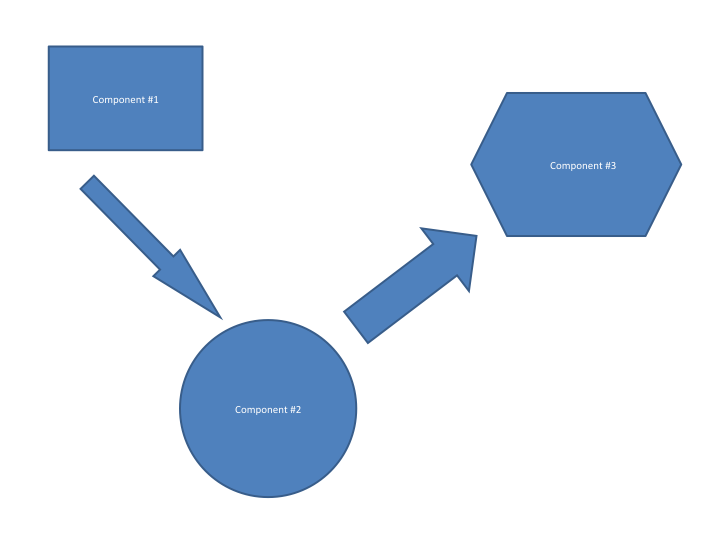
\includegraphics[width=0.75\textwidth]{./diagram}
\end{center}
\caption{A sample figure .... System Diagram \label{systemdiagram}}
\end{figure}

\section{Technologies Overview}
The primary Technologies for this projects are as follows:

\begin{enumerate}
\item Xcode and Visual Studio - Xcode and MSVS are the primary development IDEs for this project. Of the two the one the group used the most was visual studio so we could develop on the machines provided by the school.
\item Python - the primary programming language for the project
\item PHP - primary language for student web interface
\item PyQt and Qt Designer - Gui package and development environment 
\item MySQL - MySQL provides the database and relational quires to manage the data and organize it within the system.
\end{enumerate}


These technologies were selected after a first research sprint where research into programming language, GUI, and database options were selected. A brief description                    of the research can be found in the sprint 1 report or the first prototype sections of this document.